% Options for packages loaded elsewhere
\PassOptionsToPackage{unicode}{hyperref}
\PassOptionsToPackage{hyphens}{url}
%
\documentclass[
  english,
  man,mask,floatsintext]{apa6}
\usepackage{amsmath,amssymb}
\usepackage{lmodern}
\usepackage{ifxetex,ifluatex}
\ifnum 0\ifxetex 1\fi\ifluatex 1\fi=0 % if pdftex
  \usepackage[T1]{fontenc}
  \usepackage[utf8]{inputenc}
  \usepackage{textcomp} % provide euro and other symbols
\else % if luatex or xetex
  \usepackage{unicode-math}
  \defaultfontfeatures{Scale=MatchLowercase}
  \defaultfontfeatures[\rmfamily]{Ligatures=TeX,Scale=1}
\fi
% Use upquote if available, for straight quotes in verbatim environments
\IfFileExists{upquote.sty}{\usepackage{upquote}}{}
\IfFileExists{microtype.sty}{% use microtype if available
  \usepackage[]{microtype}
  \UseMicrotypeSet[protrusion]{basicmath} % disable protrusion for tt fonts
}{}
\makeatletter
\@ifundefined{KOMAClassName}{% if non-KOMA class
  \IfFileExists{parskip.sty}{%
    \usepackage{parskip}
  }{% else
    \setlength{\parindent}{0pt}
    \setlength{\parskip}{6pt plus 2pt minus 1pt}}
}{% if KOMA class
  \KOMAoptions{parskip=half}}
\makeatother
\usepackage{xcolor}
\IfFileExists{xurl.sty}{\usepackage{xurl}}{} % add URL line breaks if available
\IfFileExists{bookmark.sty}{\usepackage{bookmark}}{\usepackage{hyperref}}
\hypersetup{
  pdftitle={No meaningful effects of COVID-19 related social media use on well-being},
  pdflang={en-EN},
  pdfkeywords={COVID-19, Coronavirus, well-being, affect, life satisfaction, social media use, news use, communication, random effects within between model, panel study, longitudinal.},
  hidelinks,
  pdfcreator={LaTeX via pandoc}}
\urlstyle{same} % disable monospaced font for URLs
\usepackage{graphicx}
\makeatletter
\def\maxwidth{\ifdim\Gin@nat@width>\linewidth\linewidth\else\Gin@nat@width\fi}
\def\maxheight{\ifdim\Gin@nat@height>\textheight\textheight\else\Gin@nat@height\fi}
\makeatother
% Scale images if necessary, so that they will not overflow the page
% margins by default, and it is still possible to overwrite the defaults
% using explicit options in \includegraphics[width, height, ...]{}
\setkeys{Gin}{width=\maxwidth,height=\maxheight,keepaspectratio}
% Set default figure placement to htbp
\makeatletter
\def\fps@figure{htbp}
\makeatother
\setlength{\emergencystretch}{3em} % prevent overfull lines
\providecommand{\tightlist}{%
  \setlength{\itemsep}{0pt}\setlength{\parskip}{0pt}}
\setcounter{secnumdepth}{-\maxdimen} % remove section numbering
% Make \paragraph and \subparagraph free-standing
\ifx\paragraph\undefined\else
  \let\oldparagraph\paragraph
  \renewcommand{\paragraph}[1]{\oldparagraph{#1}\mbox{}}
\fi
\ifx\subparagraph\undefined\else
  \let\oldsubparagraph\subparagraph
  \renewcommand{\subparagraph}[1]{\oldsubparagraph{#1}\mbox{}}
\fi
% Manuscript styling
\usepackage{upgreek}
\captionsetup{font=singlespacing,justification=justified}

% Table formatting
\usepackage{longtable}
\usepackage{lscape}
% \usepackage[counterclockwise]{rotating}   % Landscape page setup for large tables
\usepackage{multirow}		% Table styling
\usepackage{tabularx}		% Control Column width
\usepackage[flushleft]{threeparttable}	% Allows for three part tables with a specified notes section
\usepackage{threeparttablex}            % Lets threeparttable work with longtable

% Create new environments so endfloat can handle them
% \newenvironment{ltable}
%   {\begin{landscape}\begin{center}\begin{threeparttable}}
%   {\end{threeparttable}\end{center}\end{landscape}}
\newenvironment{lltable}{\begin{landscape}\begin{center}\begin{ThreePartTable}}{\end{ThreePartTable}\end{center}\end{landscape}}

% Enables adjusting longtable caption width to table width
% Solution found at http://golatex.de/longtable-mit-caption-so-breit-wie-die-tabelle-t15767.html
\makeatletter
\newcommand\LastLTentrywidth{1em}
\newlength\longtablewidth
\setlength{\longtablewidth}{1in}
\newcommand{\getlongtablewidth}{\begingroup \ifcsname LT@\roman{LT@tables}\endcsname \global\longtablewidth=0pt \renewcommand{\LT@entry}[2]{\global\advance\longtablewidth by ##2\relax\gdef\LastLTentrywidth{##2}}\@nameuse{LT@\roman{LT@tables}} \fi \endgroup}

% \setlength{\parindent}{0.5in}
% \setlength{\parskip}{0pt plus 0pt minus 0pt}

% Overwrite redefinition of paragraph and subparagraph by the default LaTeX template
% See https://github.com/crsh/papaja/issues/292
\makeatletter
\renewcommand{\paragraph}{\@startsection{paragraph}{4}{\parindent}%
  {0\baselineskip \@plus 0.2ex \@minus 0.2ex}%
  {-1em}%
  {\normalfont\normalsize\bfseries\itshape\typesectitle}}

\renewcommand{\subparagraph}[1]{\@startsection{subparagraph}{5}{1em}%
  {0\baselineskip \@plus 0.2ex \@minus 0.2ex}%
  {-\z@\relax}%
  {\normalfont\normalsize\itshape\hspace{\parindent}{#1}\textit{\addperi}}{\relax}}
\makeatother

% \usepackage{etoolbox}
\makeatletter
\patchcmd{\HyOrg@maketitle}
  {\section{\normalfont\normalsize\abstractname}}
  {\section*{\normalfont\normalsize\abstractname}}
  {}{\typeout{Failed to patch abstract.}}
\patchcmd{\HyOrg@maketitle}
  {\section{\protect\normalfont{\@title}}}
  {\section*{\protect\normalfont{\@title}}}
  {}{\typeout{Failed to patch title.}}
\makeatother
\keywords{COVID-19, Coronavirus, well-being, affect, life satisfaction, social media use, news use, communication, random effects within between model, panel study, longitudinal.}
\usepackage{lineno}

\linenumbers
\usepackage{csquotes}
\setlength{\parskip}{0em}
\raggedbottom
\note{\clearpage}
\ifxetex
  % Load polyglossia as late as possible: uses bidi with RTL langages (e.g. Hebrew, Arabic)
  \usepackage{polyglossia}
  \setmainlanguage[]{english}
\else
  \usepackage[main=english]{babel}
% get rid of language-specific shorthands (see #6817):
\let\LanguageShortHands\languageshorthands
\def\languageshorthands#1{}
\fi
\ifluatex
  \usepackage{selnolig}  % disable illegal ligatures
\fi
\newlength{\cslhangindent}
\setlength{\cslhangindent}{1.5em}
\newlength{\csllabelwidth}
\setlength{\csllabelwidth}{3em}
\newenvironment{CSLReferences}[2] % #1 hanging-ident, #2 entry spacing
 {% don't indent paragraphs
  \setlength{\parindent}{0pt}
  % turn on hanging indent if param 1 is 1
  \ifodd #1 \everypar{\setlength{\hangindent}{\cslhangindent}}\ignorespaces\fi
  % set entry spacing
  \ifnum #2 > 0
  \setlength{\parskip}{#2\baselineskip}
  \fi
 }%
 {}
\usepackage{calc}
\newcommand{\CSLBlock}[1]{#1\hfill\break}
\newcommand{\CSLLeftMargin}[1]{\parbox[t]{\csllabelwidth}{#1}}
\newcommand{\CSLRightInline}[1]{\parbox[t]{\linewidth - \csllabelwidth}{#1}\break}
\newcommand{\CSLIndent}[1]{\hspace{\cslhangindent}#1}

\title{No meaningful effects of COVID-19 related social media use on well-being}
\author{Tobias Dienlin\textsuperscript{1}}
\date{}


\shorttitle{COVID-19 related social media use and well-being}

\authornote{

Tobias Dienlin, Department of Communication, University of Vienna.

Correspondence concerning this article should be addressed to Tobias Dienlin, University of Vienna, Department of Communication, 1090 Vienna, Austria. E-mail: \href{mailto:tobias.dienlin@univie.ac.at}{\nolinkurl{tobias.dienlin@univie.ac.at}}

}

\affiliation{\vspace{0.5cm}\textsuperscript{1} University of Vienna}

\abstract{
In times of crisis such as the Corona pandemic citizens need to stay informed about recent events, the latest political decisions, or mandatory protection measures. To this end, many people use various types of media, and increasingly social media. However, because social media are particularly engaging, some find it hard to disconnect and cannot stop `doomscrolling.' In this preregistered study, I investigate whether using social media for COVID-19 related reasons might put personal well-being at risk. To answer this question I analyzed data from the Austrian Corona Panel Project, which consists of 24 waves with overall 3,018 participants. I ran three random effects within between models, controlling for several stable and varying confounders Results showed that the effects of COVID-19 related social media use on well-being were very small, arguably too small to matter. The findings suggest that fears that social media use during times of crisis impairs well-being are likely to be unfounded.
}



\begin{document}
\maketitle

During the COVID-19 pandemic,
numerous events unfolded in quick succession.
Several open questions emerged.
How dangerous is the virus?
Is it spreading in my region?
How is it transmitted, and how can I protect myself?
Because for many it was (and still is) a matter of life or death, people aimed to stay informed regarding the latest developments.
Governments around the world implemented safety measures, such as wearing masks, keeping physical distance, or enforcing lockdowns.
In this extraordinary situation, many people used media excessively to attain information, and especially social media were at an all time high (Statista, 2021).

Some people could not stop using social media to learn about COVID-19 related news.
A new phenomenon termed ``doomscrolling'' emerged:
Users were glued to their screens and found it hard to pursue other relevant activities such as working, taking a break, or looking after their children (Klein, 2021).
As doomscrolling increased it became doubtful whether such social media is helpful, or whether it created an additional burden on mental health (Sandstrom, Buchanan, Aknin, \& Lotun, 2021).
These concerns seem justified:
A study with 6,233 people from Germany that was conducted during the pandemic found that ``{[}f{]}requency, duration and diversity of media exposure were positively associated with more symptoms of depression'' (Bendau et al., 2021, p. 283).

As a result, with this study I want to build on this research and investigate whether or not COVID-19 related social media use affected well-being during the pandemic.
To this end, I analyzed a large-scale panel study from the Austrian Corona Panel Project (Kittel et al., 2020).
The panel consists of 24 waves and has an overall sample size of 3018.
The panel study collected a large number of psychological and demographic variables.
I explicitly aimed to investigate the causal effects of COVID-19 related social media use on well-being.

\hypertarget{defining-well-being-and-media-use}{%
\subsection{Defining Well-being and Media Use}\label{defining-well-being-and-media-use}}

The underlying theories that guided the selection of variables for my analysis are the two-continua model of mental health (Greenspoon \& Saklofske, 2001) and the hierarchical taxonomy of computer-mediated communication (Meier \& Reinecke, 2020).
According to the two-continua model, mental health consists of (a) psychopathology and (b) well-being.
Well-being can be differentiated into subjective and psychological well-being (Diener, Lucas, \& Oishi, 2018).
Whereas subjective well-being emphasizes hedonic aspects such as happiness and joy, psychological well-being addresses eudaimonic aspects such as fulfillment and meaning.
Subjective well-being is primarily about achieving positive affect and avoiding negative affect.
One of the most prominent indicators of well-being is life satisfaction.
In my view, life satisfaction is best thought of as a meta concept that combines psychological and subjective well-being, because it represents a general appraisal of one's life.
Notably, life satisfaction is stable and fluctuates only little, whereas it's the exact opposite for affect (Dienlin \& Johannes, 2020).
To capture well-being in this study I thus build on life satisfaction, positive affect, and negative affect.
Together, this should provide an encompassing perspective on potential media effects.

The hierarchical taxonomy of computer-mediated communication differentiates six levels of how people engage with digital technology.
First, the device (e.g., smartphone); second, the type of application (e.g., social networking site); third, the branded application (e.g., Twitter); fourth, the feature (e.g., status post); fifth, the interaction (e.g., one-to-many); and sixth, the message (e.g., content) (Meier \& Reinecke, 2020).
Whereas the first four levels focus on the \emph{channel}, the last two address the \emph{type} of communication.
To measure social media use for the consumption of COVID-19 related news and topics, I here employ both the channel and the type of communication perspective, which together provides a nuanced understanding of communication.

First, I investigate how different types of communication affect well-being.
Specifically, I differentiate between active and passive use.
I distinguish (a) \emph{reading} (passive), \emph{posting} (active), and \emph{liking and sharing} COVID-19 related posts (both active and passive).
Second, I analyze how using the most prominent branded applications affects well-being, and whether this effect changes across applications.
Branded apps are separate entities with potentially divergent effects.
Twitter might have a different effect as compared to WhatsApp because of their respective affordances.
For example, Waterloo, Baumgartner, Peter, and Valkenburg (2018) found that it's more adequate to express negative emotions on WhatsApp than on Twitter or on Instagram.
The branded applications investigated here are Facebook, Twitter, Instagram, WhatsApp, and YouTube.
Worth noting, this study is not about \emph{general} social media use during times of COVID, but on social media use \emph{focused} on COVID-19 related content.
Examples of such media use include posting thoughts about the pandemic or retweeting COVID-19 related news.

\hypertarget{effects-of-social-media-on-well-being}{%
\subsection{Effects of Social Media on Well-Being}\label{effects-of-social-media-on-well-being}}

So far, there is only little empirical research on COVID-19 related social media use on well-being.
In their study on the relations between media use and mental health during the pandemic, Bendau et al. (2021) found that people who used social media as a primary source of information reported on average ``significantly more unspecific anxiety and depression {[}{]} and significantly more specific COVID-19 related anxiety symptoms'' (p.~288).
Eden, Johnson, Reinecke, and Grady (2020) analyzed the media use of 425 US college students during the first wave of the pandemic, finding both positive and negative relations with well-being.
In a sample of 312 respondents collected via Amazon Mechanical Turk, Choi and Choung (2021) reported that people who used media to attain information were more lonely and less satisfied with their lives.
Stainback, Hearne, and Trieu (2020) analyzed a large-scale study with 11,537 respondents from the US and found that increased COVID-19 media consumption was related to more psychological distress.
Together, the literature emphasizes potentially negative effects of social media as news use (see also Liu \& Tong, 2020; Riehm et al., 2020).
However, note that all of these findings represent between-person relations stemming from cross-sectional data (see below).
We therefore don't know whether the differences in mental health and well-being are due to social media use or due to other third variables, such as age, health, employment, or education.

The question of whether and how social media use affects well-being \emph{in general}, on the other hand, is well-researched.
This also holds true for the different types of communication such as active or passive use.
A meta review (i.e., an analysis of meta-analyses) found that the relation between social media use and well-being is likely in the negative spectrum but very small (Meier \& Reinecke, 2020)---potentially too small to matter.
What determines whether or not an effect is considered small or trivial?
As a starting point, we could refer to standardized effect sizes.
According to Cohen (1992), small effect sizes start at \emph{r} = .10.
And indeed, several if not most of the current meta-analyses find effect sizes below that threshold (Ferguson et al., 2021; Huang, 2017; Meier \& Reinecke, 2020).

These overviews are well aligned with several individual studies employing advanced methods (Keresteš \& Štulhofer, 2020; Orben, Dienlin, \& Przybylski, 2019; Przybylski, Nguyen, Law, \& Weinstein, 2021; Schemer, Masur, Geiß, Müller, \& Schäfer, 2021).
For example, Beyens, Pouwels, Driel, Keijsers, and Valkenburg (2021) reported that although for some users (roughly one quarter) the effects of social media use on well-being were negative, for almost the same number of users they were positive, while for the rest the effects were neutral.
In conclusion, most effects are likely somewhere between trivial and small.
I therefore expect that also in the case of COVID-19 related social media use effects will be trivial to small.

From a theoretical perspective, how could we explain whether COVID-19 related social media use might affect well-being?
In what follows, I outline potential arguments as to why the effect might be positive or negative, direct or indirect, or nonexistent.
In advance, there does not seem to be a clear winner, and it's likely that both positive and negative effects are equally strong.

First, one could assume a \emph{direct} negative effect on well-being, and especially on positive or negative affect, which is more volatile and fluctuating.
Dangers, inequalities, corruption---these were the headlines during the pandemic across many countries worldwide.
If one learns about such events, the initial reaction might be shock, fear, or dismay.
Repeatedly consuming such news can be depressing, perhaps even changing some general perspectives on life.
That said, because not all news was negative, and because many people showed solidarity and compassion, there was also positive and uplifting content, potentially compensating for the negative effects.

There could also be \emph{indirect} effects.
When doomscrolling, users are captivated to such an extent that they cannot stop using social media.
For example, during the pandemic social media use was at an all-time high in the US (Statista, 2021).
In general, as has been expressed by many before, it is most likely that moderate social media use is not detrimental (Orben, 2020).
Overuse, however, might be more critical, and several studies have shown more pronounced negative effects for extreme users (Przybylski \& Weinstein, 2017).
To explain, overuse likely impairs well-being if it replaces meaningful or functional activities such as meeting others, working, actively relaxing, or exercising.
So if a society collectively overuses social media when doomscrolling, there is potential for negative effects.

On the other hand, one can make the case that overuse might also be beneficial, especially in times of a pandemic---even if the use is mainly COVID-19 related.
Exchanging COVID-19 related messages with friends via WhatsApp might replace the in-person contact one would have otherwise, but which is literally impossible at the time.
In situations where meaningful and functional activities are prohibited, using social media to exchange about COVID-19 related topics might be not the worst idea.
Besides, given that nowadays a large number of experts, scientists, and politicians converse directly on social media, one can get first-hand high quality information on current developments.

Together, the strongest argument to me is that \emph{in general} the effects of social media on well-being are, on average, small at best.
Because this study only looks at \emph{one part} of social media use---namely, COVID-19 related interactions---it is very focused, diminishing the overall potential of the effects even further.
Whether or not using social media for COVID-19 related aspects is detrimental during a pandemic is also not entirely clear.
Therefore, I expect that COVID-19 related communication on social media does not affect well-being in a meaningful or relevant way.

\begin{quote}
Hypothesis: The within-person effects of all types of COVID-19 related social media use on all types of well-being indicators---while controlling for several stable and varying covariates such as sociodemographic variables and psychological dispositions---will be trivial.
\end{quote}

\hypertarget{current-study}{%
\section{Current Study}\label{current-study}}

\hypertarget{smallest-effect-size-of-interest}{%
\subsection{Smallest Effect Size of Interest}\label{smallest-effect-size-of-interest}}

Testing this hypothesis, however, is not trivial.
First, in contrast to most hypotheses typically posited in the social sciences it implicitly contains an effect size, a so-called smallest effect size of interest (SESOI).
Effectively testing this hypothesis necessitates defining what's considered a ``trivial effect size'' and what's not.
Above I already referred to standardized effect sizes.
However, standardized effect sizes should only be a first step toward evaluating an effect's relevance (Baguley, 2009).
Standardized effect sizes are determined by a sample's variance,\footnote{Consider the effect size Cohen's \emph{d}: The mean's of the two groups that are to be compared are subtracted from one another and then divided by the sample's standard deviation (Cohen, 1992). Hence, if there is more deviation/variance in a sample, the effect size decreases, even if the difference of the group's means stays the same.} which is problematic:
The question of whether or not social media use affects a particular person in a relevant way should not depend on the variance in the sample in which that person's data were collected.
Instead, it should depend on absolute criteria.

What could be a minimally interesting, nontrivial effect?
Because this is a normative and ultimately philosophical question, there can never be a clear, single, or unanimous answer.
However, it is still necessary and helpful to try provide such a plausible benchmark.
I therefore suggest the following SESOI for this research question:

\begin{quote}
SESOI: If a heavy user of COVID-19 related social media news suddenly \emph{stops} using social media altogether, this should have a \emph{noticeable} impact on their overall well-being.
\end{quote}

What does this mean practically and how can it be operationalized?
In this study, COVID-19 related social media use was measured on a 5-point scale, ranging from 1 = \emph{never} to 5 = \emph{several times a day}.
Thus, a change of four units in social media use (e.g., a complete stop) should correspond to a noticeable change in well-being.
But what's a noticeable change in well-being?
According to Norman, Sloan, and Wyrwich (2003), people can reliably distinguish \emph{seven} levels of satisfaction with health.
So if satisfaction is measured on a 7-point scale, we would state that a four unit change in social media use should result in a one unit change in life satisfaction.
(For more information, see Method section ``Inference criteria.'')

\hypertarget{causality}{%
\subsection{Causality}\label{causality}}

The hypothesis explicitly states a causal effect.
In non-experimental studies, longitudinal designs help investigate causality.
Using longitudinal designs alone, however, is not sufficient for establishing correct causal statements (Rohrer \& Murayama, 2021).
In addition, we for example also need to control for confounding third variables, and importantly also for \emph{varying} third variables.

To illustrate, consider the following example.
Imagine that a person suddenly starts using social media much more than usual, and then after some time becomes less satisfied with their life.
Eventually, use and life satisfaction return to prior levels.
If this happens to several people at the same time, in a longitudinal study we could then observe a significant effect of social media use on life satisfaction.
However, it could also be the case that during the study there was a major exogenous event (say, a pandemic), which caused large parts of the working population to loose their jobs.
Hence, the causal effect reported above was confounded, because in reality it was the pandemic that caused both social media use to rise and life satisfaction to go down.

Thus, only when controlling for \emph{all} relevant confounders, we can correctly estimate causality without bias (Rohrer, 2018).
Obviously, we can never be entirely sure to have included all confounders, which makes absolute statements regarding causality virtually impossible.
In addition, when determining the overall causal effect, we need to make sure \emph{not} to control for mediating variables (Rohrer, 2018), for doing so would bias our assessment of the causal effect.
Complicating matters further, it is often unclear if a variable is a mediator or a confounder.\footnote{In addition, there also exist colliders, which I don't discuss here and which complicate the issue even further (Rohrer, 2018).}
However, despite all these caveats, when controlling for relevant variables (that aren't mediators), we can be much more certain that we measured causality correctly.
The aim should therefore be to collect as many varying and nonvarying confounders as possible (which it seems is seldom done in our field), while knowing that absolute certainty regarding causality cannot be reached.

When searching for suitable candidates for confounders, we should look out for variables that affect both media use and well-being.
Controlling for these factors isolates the actual effect of social media use on well-being.
We can also control for variables that affect only social media use or well-being.
However, in doing so not much is gained or lost, because the effects of social media use would remain virtually the same (Kline, 2016; but see McElreath, 2021).

In this study, I hence plan to control for the following variables, which either have already been shown to affect both social media use and well-being or which are likely to do so, and which also are not mediators:
gender, age, education, Austria country of birth, Austria country of birth of parents, text-based news consumption, video-based news consumption, residency Vienna, household size, health, living space, access to garden, access to balcony, employment, work hours per week, being in home-office, household income, outdoor activities, satisfaction with democracy, disposition to take risks, and locus of control.
I will not control for variables such as trust in institutions or trust in media, because these variables might be influenced by social media use to a meaningful extent.

Next to including covariates, it is now increasingly understood that causal effects should be analyzed from an internal, within-person perspective (Hamaker, 2014).
If a specific person changes their media diet, we need to measure how this behavior affects \emph{their own} well-being.
Between-person comparisons from cross-sectional data, where participants are interviewed only once, cannot provide such insights.
In this study, I hence differentiate between-person relations from within-person effects.
And as explicated above, to test the hypothesis I thus consider only the within-person effects.

Finally, one precondition of causality is temporal order.
The cause needs to precede the effect.
Finding the right interval between cause and effect is crucial.
For example, if we want to measure the effect of alcohol consumption on driving performance, it makes a big difference if driving performance is measured one minute, one hour, one day, or one week after consumption.
If variables are stable, longer intervals are needed; if they fluctuate, shorter intervals.
In the case of well-being, we need shorter intervals for affect and longer ones for life satisfaction.
Still, choosing the right interval is challenging, because especially short intervals are hard to implement in practice and often require advanced methods such as experience sampling (also known as in situ measurement or ambulant assessment) (Schnauber-Stockmann \& Karnowski, 2020).

In this study, I therefore adopt an intermediate perspective.
I analyze if when a person changes their social media diet, are there simultaneous changes in their well-being?
When additionally controlling for both stable and varying confounders, we can then be more sure that the effect is indeed causal.

\hypertarget{method}{%
\section{Method}\label{method}}

In this section I describe the preregistration and how I determined the sample size, data exclusions, the analyses, and all measures in the study.

\hypertarget{preregistration}{%
\subsection{Preregistration}\label{preregistration}}

The hypotheses, the sample, the measures, the analyses, and the inference criteria (SESOI, p-value) were preregistered on the Open Science Framework.
The (anonymous) preregistration can be accessed here: \url{https://osf.io/87b24/?view_only=b2289b6fec214fa88ee75a18d45c18f3}.
Because in this study I analyzed data from an already existing large-scale data set, all of these steps were done prior to accessing the data.
The preregistration was designed on the basis of the panel documentation online (Kittel et al., 2020).
In some cases I could not execute the analyses as I had originally planned, for example because some properties of the variables only became apparent when inspecting the actual data.
The most relevant deviations are reported below, and a complete list of all changes can be found in the online \href{https://tdienlin.github.io/Austrian_Corona_Panel/index.html}{companion website} (\url{https://tdienlin.github.io/Austrian_Corona_Panel/index.html}).

\hypertarget{sample}{%
\subsection{Sample}\label{sample}}

The data come from the Austrian Corona Panel Project (Kittel et al., 2021).
The study was conducted between March 2020 and October 2021.
It contains 26 waves, and at the time of writing the first 24 waves were available for download.
Each wave consists of at least 1,500 respondents.
The overall sample size was \emph{N} = 3,018, and 72,432 observations were collected.
Panel mortality was compensated through a continuous acquisition of new participants.
All respondents needed to have access to the internet (via computer or mobile devices such as smartphones or tablets).
They were sampled from a pre-existing online access panel provided by the company Marketagent, Austria.
Respondents were asked and incentivized with 180 credit points to participate in each wave of the panel.

The sample was representative of the Austrian population in terms of age, gender, region/state, municipality size, and educational level.
In order to participate in the study, the respondents needed to be Austrian residents and had to be at least 14 years of age.
The study received IRB approval from the University of Vienna.
The average age was 42 years, 49 percent were male, 14 percent had a University degree, and 5 percent were currently unemployed.

\hypertarget{inference-criteria}{%
\subsection{Inference criteria}\label{inference-criteria}}

Because the data were analyzed post-hoc, no a-priori sample size planning on the basis of power analyses was conducted.
The sample is large, and it is hence well-equipped reliably to detect also small effects.
In addition, because such large samples easily generate significant \emph{p}-values even for very small effects, it helps that the hypotheses were tested with a smallest effect size of interest-approach.
To this end, I adopted the interval testing approach as proposed by Dienes (2014).
On the basis of the SESOI, I then defined a null region.
In what follows, I explain how I determined the SESOI and the null region.

In this study, life satisfaction was measured on an 11-point scale.
If people can reliably differentiate 7 levels as mentioned above, this corresponds to 11 / 7 = 1.57 unit change on an 11-point scale.
Hence, a four-point change in media use (e.g., a complete stop) should result in a 1.57-point change in life satisfaction.
In a statistical regression analysis, \emph{b} estimates the change in the dependent variable if the independent variable increases by one point.
We would therefore expect a SESOI of \emph{b} = 1.57 / 4 = 0.39.
For affect, which was measured on a 5-point scale, our SESOI would be \emph{b} = 0.71 / 4 = 0.18.
Because we're agnostic as to whether the effects are positive or negative, the null region includes negative and positive effects.
Finally, in order not to exaggerate precision and to be less conservative, these numbers are reduced to nearby thresholds.\footnote{Note that other researchers also decreased or recommended decreasing thresholds for effect sizes when analyzing within-person or cumulative effects (Beyens, Pouwels, Driel, Keijsers, \& Valkenburg, 2021; Funder \& Ozer, 2019).}
Together, this leads to a null region ranging from \emph{b} = -.30 to \emph{b} = .30 for life satisfaction, and \emph{b} = -.15 to \emph{b} = .15 for positive and negative affect.

To illustrate what this means in practice, if the 95\% confidence interval falls completely within the null-region (e.g., \emph{b} = .20, {[}95\% CI: .15, .25{]}), the hypothesis that the effect is trivial is supported.
If the effects interval and the null region overlap (e.g., \emph{b} = .30, {[}95\% CI: .25, .35{]}), the hypothesis is not supported and the results are considered inconclusive, while a meaningful negative effect is rejected.
If the confidence falls completely outside of the null-region (e.g., \emph{b} = .40, {[}95\% CI: .35, .45{]}), the hypothesis is rejected and the existence of a meaningful positive effect is supported.

\hypertarget{data-analysis}{%
\subsection{Data Analysis}\label{data-analysis}}

The hypothesis was analyzed using mixed effects models, namely random effect within-between models (REWB)(Bell, Fairbrother, \& Jones, 2019).
Three models were run, one for each dependent variable.
The data were hierarchical, and responses were separately nested in participants and waves (i.e., participants and waves were implemented as random effects).
Nesting in participants allowed to separate between-person relations from within-person effects.
Nesting in waves allowed to control for general exogenous developments, such as general decreases in well-being in the population, for example due to lockdown measures.
Thus, there was no need additionally to control for specific phases or measures of the lockdown.
Predictors were modeled as fixed effects.
They included social media communication types and channels, separated into within and between-person factors, as well as stable and varying covariates.
All predictors were included simultaneously and in each of the three models.

The factorial validity of the scales were tested with confirmatory factor analyses (CFA).
Because Mardia's test showed that the assumption of multivariate normality was violated, I used the more robust Satorra-Bentler scaled and mean-adjusted test statistic (MLM) as estimator.
To avoid overfitting, I tested the scales on more liberal fit criteria (CFI \textgreater{} .90, TLI \textgreater{} .90, RMSEA \textless. .10, SRMR \textless{} .10) (Kline, 2016).
Finally, REWB-models cannot model latent variables.
To increase precision, I therefore exported factor scores from the CFAs for positive and negative affect.
Respondents who answered less than 50\% of all questions were removed.
The remaining missing responses were imputed using predictive mean matching.

For more information on the analyses, a complete documentation of the models and results, see \href{https://tdienlin.github.io/Austrian_Corona_Panel/index.html}{companion website}.

\hypertarget{measures}{%
\subsection{Measures}\label{measures}}

In what follows, I list all the variables that I analyzed.
For the variables' means, range, and variance, see Table \ref{tab:descriptives}.
For a complete list of all items and item characteristics, see \href{https://tdienlin.github.io/Austrian_Corona_Panel/index.html}{companion website}.

\hypertarget{well-being}{%
\subsubsection{Well-being}\label{well-being}}

Life satisfaction was measured with the item ``Taken everything together, how satisfied are you currently with your life?''
The response options ranged from 0 (\emph{extremely unsatisfied}) to 10 (\emph{extremely satisfied}).

To capture positive affect, respondents were asked how often in the last week they felt (a) calm and relaxed, (b) happy, and (c) full of energy.
The response options were 1 (\emph{never}), 2 (\emph{on some days}), 3 (\emph{several times per week}), 4 (\emph{almost every day}), and 5 (\emph{daily}).
The scale showed good factorial fit, \(\chi^2\)(46) = 65.30, \textit{p} = .032, cfi = 1.00, rmsea = .02, 90\% CI {[}.01, .03{]}, srmr = .01.
Reliability was high, \(\omega\) = .85.

For negative affect, respondents were asked how often in the last week they felt (a) lonely, (b) aggravated, (c) so depressed, that nothing could lift you up, (d) very nervous, (e) anxious, and (h) glum and sad.
The response options were 1 (\emph{never}), 2 (\emph{on some days}), 3 (\emph{several times per week}), 4 (\emph{almost every day}), and 5 (\emph{daily}).
The scale showed good factorial fit, \(\chi^2\)(331) = 3138.37, \textit{p} \textless{} .001, cfi = .97, rmsea = .08, 90\% CI {[}.07, .08{]}, srmr = .03.
Reliability was high, \(\omega\) = .89.

All three variables were measured on each wave.

\hypertarget{covid-19-related-social-media-use}{%
\subsubsection{COVID-19 related social media use}\label{covid-19-related-social-media-use}}

COVID-19 related social media use focused on communication \emph{types} was measured with the three dimensions of (a) reading, (b) liking and sharing, and (c) posting.
The general introductory question was ``How often during the last week have you engaged in the following activities on social media?''
The three items were ``Reading the posts of others with content on the Coronavirus,'' ``When seeing posts on the Coronavirus, I clicked `like,' `share' or `retweet','' ``I myself wrote posts on the Coronavirus on social media.''
Answer options were 1 (\emph{several times per day}), 2 (\emph{daily}), 3 (\emph{several times per week}), 4 (\emph{weekly}), 5 (\emph{never}).
The items were inverted for the analyses.

COVID-19 related social media use focused on \emph{channels} was measured with five variables.
The general introductory question was ``How often in the last week have you followed information related to the Corona-crisis on the following social media?''
The five items were (a) Facebook, (b) Twitter, (c) Instagram, (d) Youtube, and (e) WhatsApp.
Again, the answer options were 1 (\emph{several times per day}), 2 (\emph{daily}), 3 (\emph{several times per week}), 4 (\emph{weekly}), 5 (\emph{never}).
Again, the items were inverted for the analyses.

Social media use was measured for all participants on waves 1, 2, 8, 17, and 23.
Freshly recruited respondents always answered all questions on social media use.

\begin{table}[tbp]

\begin{center}
\begin{threeparttable}

\caption{\label{tab:descriptives}Descriptives of the main variables.}

\begin{tabular}{lllll}
\toprule
 & \multicolumn{1}{c}{sd} & \multicolumn{1}{c}{min} & \multicolumn{1}{c}{max} & \multicolumn{1}{c}{mean}\\
\midrule
Well-being &  &  &  & \\
\ \ \ Life satisfaction & 1.68 & 6.38 & 6.81 & 6.59\\
\ \ \ Positive affect & 0.57 & 3.05 & 3.28 & 3.15\\
\ \ \ Negative affect & 0.39 & 1.66 & 1.81 & 1.73\\
Social media use &  &  &  & \\
\ \ \ Read & 1.03 & 2.10 & 2.92 & 2.43\\
\ \ \ Like \& share & 0.87 & 1.61 & 1.92 & 1.78\\
\ \ \ Posting & 0.63 & 1.33 & 1.46 & 1.39\\
Social media channel &  &  &  & \\
\ \ \ Facebook & 0.96 & 2.34 & 2.68 & 2.45\\
\ \ \ Twitter & 0.52 & 1.16 & 1.72 & 1.37\\
\ \ \ Instagram & 0.83 & 1.84 & 2.66 & 2.09\\
\ \ \ WhatsApp & 1.23 & 2.28 & 2.62 & 2.45\\
\ \ \ YouTube & 0.88 & 1.77 & 2.30 & 2.00\\
\bottomrule
\end{tabular}

\end{threeparttable}
\end{center}

\end{table}

\hypertarget{control-variables}{%
\subsubsection{Control variables}\label{control-variables}}

The effects of COVID-19 related social media use were controlled for the following stable variables:
(a) gender (female, male, diverse), (b) age, (c) education (ten options), (d) Austria country of birth (yes/no), (e) Austria parents' country of birth (no parent, one parent, both parents).
I originally planned to implement additional variables as varying covariates.
However, because they were not measured often enough or not at the time when social media use was measured, I implemented them as stable variables using their average values across all waves.
This includes (a) text-based media news consumption (five degrees), (b) video-based media news consumption (five degrees), (c) residency is Vienna (yes/no), (d) self-reported physical health (five degrees), (e) living space (eleven options), (f) access to balcony (yes/no), (g) access to garden (yes/no), (h) employment (nine options), (i) disposition to take risks (eleven degrees), and (j) locus of control (five degrees).
I also controlled for the following varying covariates: (a) five items measuring outdoor activities such as sport or meeting friends (five degrees), and (b) satisfaction with democracy (five degrees).
Because it lead to too much attrition in the sample, I did not control for (a) household size, (b) work hours per week, (c) home office, (d) household income.

\hypertarget{results}{%
\section{Results}\label{results}}

First, when looking at the variables from a descriptive perspective, we see that all well-being measures did not change substantially across the different waves of data collection.
COVID-19 related media use, however, decreased slightly at the beginning of the study and remained stable after approximately six waves.
The initial decrease might be explained by the fact that the collection of data began at the end of March 2020, hence approximately three months after the pandemic began.
It could be that after an initial uptick, COVID-19 related social media use was already declining at the time, returning to more normal levels.

\begin{figure}
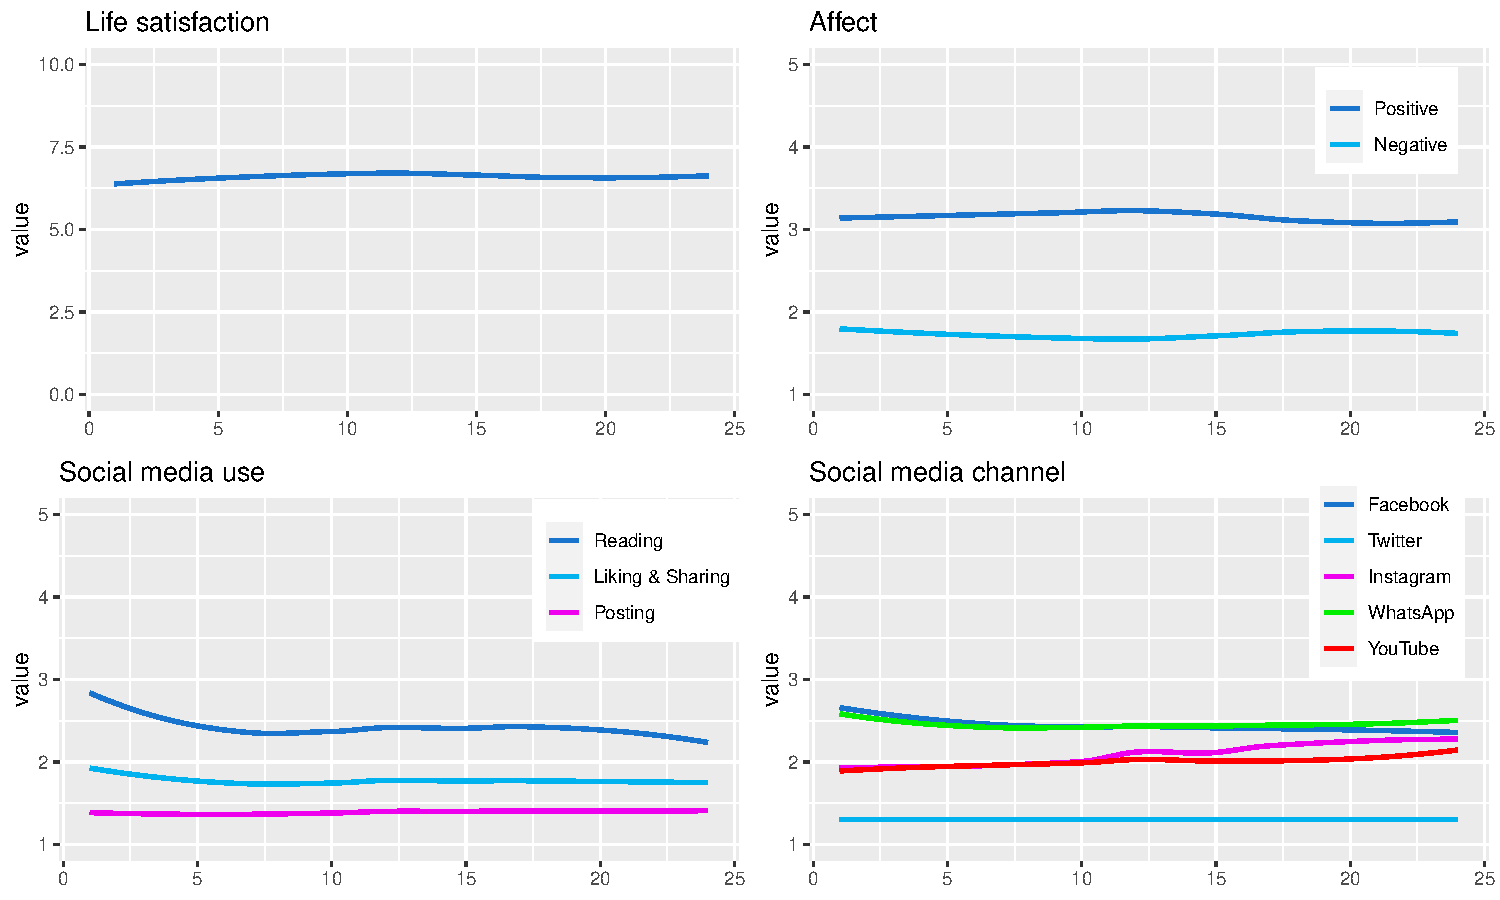
\includegraphics[width=\textwidth]{figures/fig_descriptives} \caption{Development of well-being and media use measures across the pandemic. Values obtained from mixed effect models, with participants and waves as grouping factors and without additional predictors.}\label{fig:fig-desc}
\end{figure}

\hypertarget{preregistered-analyses}{%
\subsection{Preregistered Analyses}\label{preregistered-analyses}}

The study's main hypothesis was that the effects of social media use on well-being would be trivial.
Regarding the effects of different communication \emph{types}---that is, reading vs.~sharing vs.~posting---all within-person effects fell completely within the a-priori defined null region (see Figure \ref{fig:res-activity}).
For example, respondents who used social media more frequently than usual to read about COVID-19 related topics did not show a simultaneous change in life satisfaction (\emph{b} = 0.05 {[}95\% CI -0.01, 0.1{]}).
All confidence intervals included zero; hence, all effects were also statistically non-significant.
As a result, the hypothesis was supported for all COVID-19 related types of social media communication.

\begin{figure}
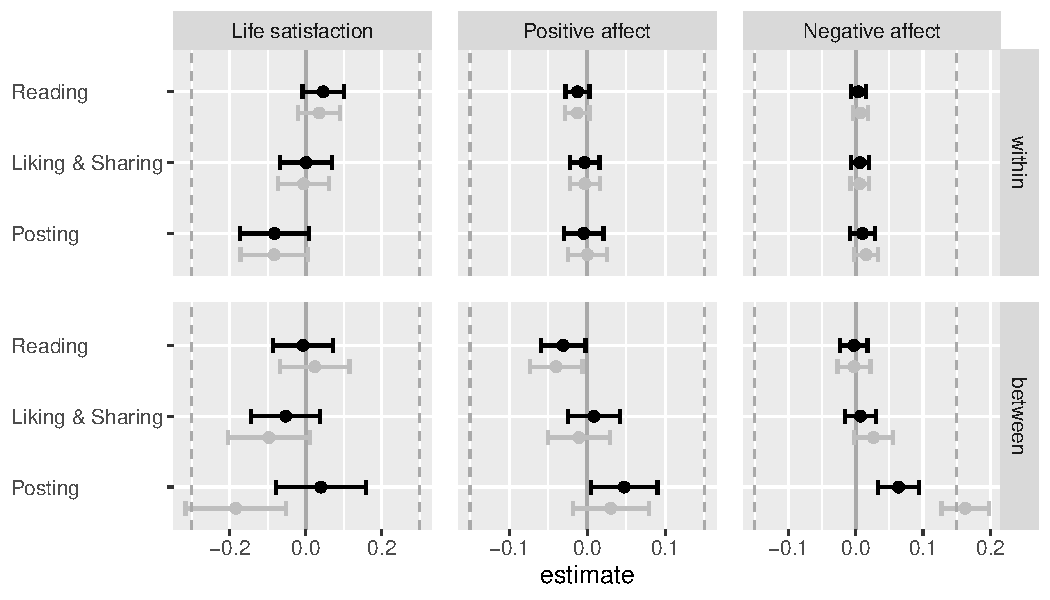
\includegraphics[width=\textwidth]{figures/fig_results_activity} \caption{The effects of various types of social media use on three indicators of well-being. The black estimates show the effects controlled for a large number of covariates (see text; preregistered); the grey estimates are without control variables (exploratory). The SESOI was \textit{b} = |0.30| for life satisfaction and \textit{b} = |0.15| for affect. Hence, all of the reported effects are considered not meaningful.}\label{fig:res-activity}
\end{figure}

Regarding between-person relations, about which no hypotheses were formulated, only three effects didn't include zero.
Respondents who across all waves used social media more frequently than others to read about COVID-19 related posts reported slightly lower levels of positive affect than others (\emph{b} = -0.03 {[}95\% CI \textgreater{} -0.01, -0.06{]}).
Respondents who across all waves used social media more frequently than others to write COVID-19 related posts reported higher levels of negative affect than others (\emph{b} = 0.06 {[}95\% CI 0.09, 0.03{]}).
Interestingly, respondents who across all waves used social media more frequently than others to write COVID-19 related posts also reported slightly higher levels of positive affect than others (\emph{b} = 0.05 {[}95\% CI 0.09, \textless{} 0.01{]}).
However, note that the effect were still completely inside of the null region, hence not large enough to be considered practically relevant.

Note that when comparing the results with and without control variables, the results differed.
For example, on the between-person level, one effect stopped being significant if controlled for additional variables.
Actively posting on social media was significantly (though not meaningfully) related to decreased life satisfaction.
However, when controlling for potential confounders, the effect became virtually zero (see Figure \ref{fig:res-channels}).

\begin{figure}
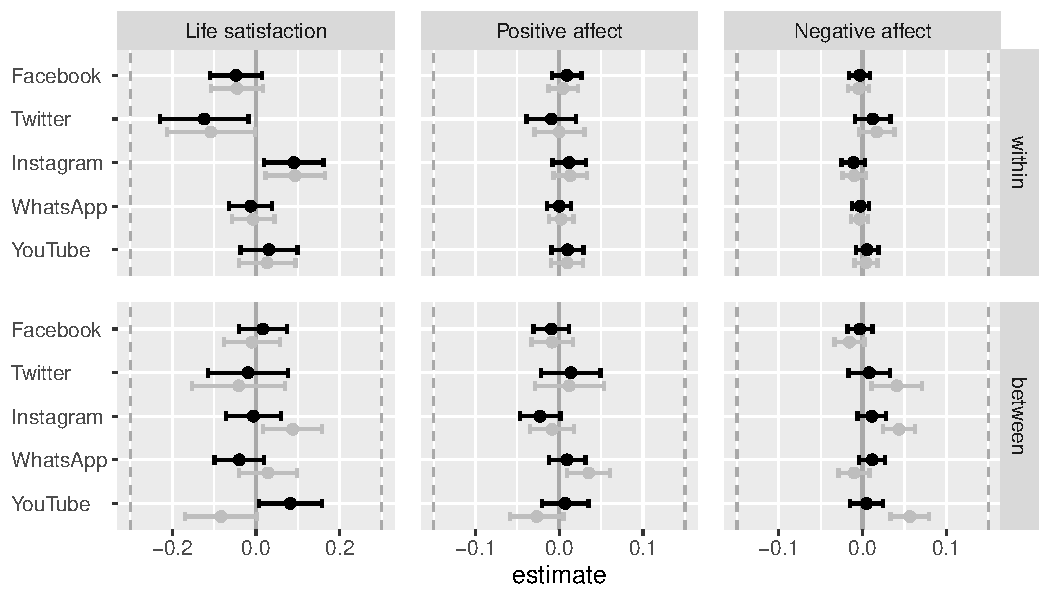
\includegraphics[width=\textwidth]{figures/fig_results_channel} \caption{The effects of using various social media applications on three indicators of well-being. The black estimates show the effects controlled for a large number of covariates (see text); the grey estimates are without control variables. The SESOI was \textit{b} = |0.30| for life satisfaction and \textit{b} = |0.15| for affect. Hence, all of the reported effects are considered not meaningful.}\label{fig:res-channels}
\end{figure}

Regarding the COVID-19 related use of social media \emph{channels}, the results were comparable (see Figure \ref{fig:res-channels}).
Changes in the frequency of using different social media channels to attain information regarding COVID-19 were unrelated to meaningful changes in well-being.
For example, respondents who used Facebook more frequently than usual to learn about COVID-19 did not show a simultaneous change in well-being (\emph{b} = -0.05 {[}95\% CI -0.11, 0.01{]}).
Only two effects differed substantially from zero.
Respondents who used Instagram more frequently than usual to attain COVID-19 related news reported slightly \emph{higher} levels of life satisfaction than usual (\emph{b} = 0.09 {[}95\% CI 0.02, 0.16{]}).
Respondents who used Twitter more frequently than usual to attain COVID-19 related news reported slightly \emph{lower} levels of life satisfaction than usual (\emph{b} = -0.12 {[}95\% CI -0.23, -0.02{]}).
However, both effects were still completely inside of the null region, hence not large enough to be considered meaningful.
In sum, the hypothesis was supported also for the COVID-19 related use of important social media channels.

In terms of between-person relations---which, again, weren't included in the hypotheses---no relations crossed the null region or fell outside of it.
Only one relation did not include zero, was hence statistically significant.
Respondents who across all waves used YouTube more frequently than others for COVID-19 related reasons reported marginally \emph{higher} levels of life satisfaction (\emph{b} = 0.08 {[}95\% CI \textless{} 0.01, 0.16{]}).
However, please note that this effect again was not large enough to be considered practically relevant.

Again, note that when comparing the results with and without control variables, the results differed.
Especially on the between-person level, altogether five effects stopped being significant if they were controlled for additional variables.
For example, using Instagram was significantly (though not meaningfully) related to increased life satisfaction.
However, when controlling for additional covariates, the effect became virtually zero (see Figure \ref{fig:res-channels}).

\hypertarget{exploratory-analyses}{%
\subsection{Exploratory Analyses}\label{exploratory-analyses}}

In what follows, I briefly report some exploratory analyses that weren't preregistered.
First, to contextualize the results reported above, and to see if other variables showed meaningful effects, I also looked at the effect sizes of selected cherry-picked covariates.
Because each variable had different response options, we would need to define a SESOI for each variable, which for reasons of scope I cannot implement here.
Therefore, I report the results of the standardized scales,
which allows for a better comparison across the differently scaled variables.
For what it's worth, as a rough estimate for the SESOI we can build on the typical convention that small effects start at \emph{r} = \textbar.10\textbar.
The results showed that several effects fell outside of the SESOI, were hence considered meaningful.
This includes for example internal locus of control, health, satisfaction with democracy, or exercising.
For an overview, see Figure \ref{fig:res-control}.

\begin{figure}
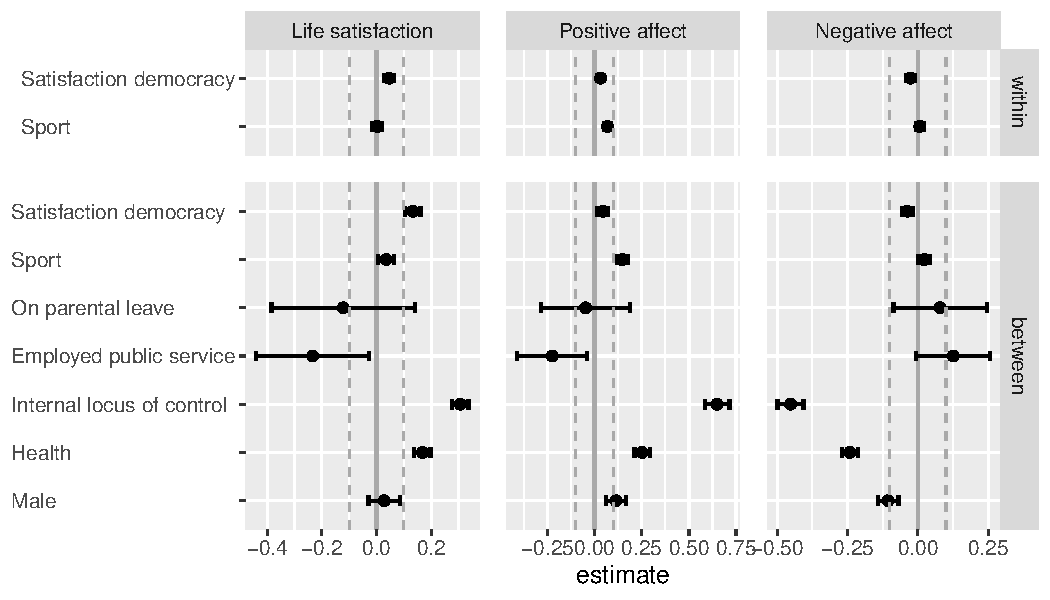
\includegraphics[width=\textwidth]{figures/fig_results_control_std} \caption{Results of selected covariates. All variables were standardize except 'Male'  and ‘Employed in public service' because there were binary.}\label{fig:res-control}
\end{figure}

To find out whether my inferences were robust across legitimate (though arguably inferior) alternative analyses, I reran the analyses also using standardized estimates, mean scores instead of factor scores, and with a data set where missing data were not imputed.
The results were virtually the same.
For example, all standardized COVID-19 related types of social media use or channels were not significantly larger than a SESOI of \(\beta\) = \textbar.10\textbar.
The additional analyses are reported in the \href{https://tdienlin.github.io/Austrian_Corona_Panel/analyses_additional.html}{companion website}.

\hypertarget{discussion}{%
\section{Discussion}\label{discussion}}

In this study I analyzed the effects of COVID-19 related social media use on well-being.
The data come from a panel study with 24 waves and are representative of the Austrian population.
In a random effects model I separated between person relations from within-person effects and controlled for a large number of both stable and varying covariates, aiming to assess causality.
The results showed that within-person effects were trivial.
People who used social media more than usual to learn about COVID-19 didn't show meaningful changes in their well-being.

The results imply that COVID-19 related social media use does not seem to be particularly relevant for well-being.
Other factors among the third variables that were measured revealed larger effects or relations, suggesting that well-being is determined by alternative aspects such as health, satisfaction with democracy, locus of control, or exercising.
According to this study, popular fears that ``doomscrolling'' or overusing social media during times of crises don't seem to be justified.

On the one hand, the results are not aligned with several recent studies analyzing similar or closely related research questions.
This includes a study by Bendau et al. (2021), which showed negative relations between social media and well-being.
However, note that Bendau et al. (2021) analyzed cross-sectional data on a between-person level while not controlling for third variables, which is not optimal for investigating causal effects.
On the other hand, the results are well-aligned with recent studies and meta-analyses analyzing the effects of social media use from a more general perspective or from a somewhat different angle.
These studies have found that the effects of various types of social media use on several well-being indicators are small at best, often too small to matter (Ferguson et al., 2021; Meier \& Reinecke, 2020; Orben, 2020), which echoes the results obtained here.

If anything, two preliminary and subtle trends can be observed.
First, of all the three COVID-19 related social media activities, people who read about the pandemic more than others showed decreased levels of positive affect, and people who actively posted about the pandemic more than others showed slightly increased levels of negative affect.
On the other hand, people who posted more about COVID-19 also showed slightly higher levels of positive affects, so taken together the results are ambivalent.
Second, in terms of media channels, using Twitter more than usual was related to slightly decreased levels of life satisfaction.
Twitter is considered to have more negative affordances and tonality as compared to other networks such as Instagram (Waterloo, Baumgartner, Peter, \& Valkenburg, 2018), which might help explain the results.
Instagram, on the other hand, was related to slightly increased simultaneous levels of life satisfaction.
To speculate, the often-criticized positivity bias on Instagram might have been somewhat beneficial in times of the pandemic.
That said, all these effects were still very small and arguably too small to matter.
But future research might elaborate on these specific relations to probe their stability and relevance.

Finally, another interesting observation is that life satisfaction was remarkably stable.
Hence, even in times of a pandemic, it seems that such broad assessment of life vary only mildly.
This supports the hypothesis that life satisfaction seems to be determined largely by stable factors such as one's genes (Brown \& Rohrer, 2019).

\hypertarget{limitations}{%
\subsection{Limitations}\label{limitations}}

The current study analyzed whether changes in media use were related to changes in well-being, while controlling for several potential confounders.
Together, this allows for an improved perspective on assessing causality.
That said, causality necessitates temporal order, and the cause needs to precede the effect.
Regarding media use, such effects often happen immediately or shortly after use, necessitating intervals in the hours, minutes, or even seconds.
In many cases only experience sampling studies asking users in the very moment can produce such knowledge.
However, even then we don't know for certain if we actually measured the right interval.
Effects depend on the intensity of use or the length of the interval, and to borrow the words from Rohrer and Murayama (2021), there is no such thing as ``the'' effect of social media use on well-being.
Hence, to document how effects unfold, future research needs to employ different study designs probing different time lags.
In addition, more thought needs to be invested in what relevant stable and varying factors we should include as control variables, and I hope this study provides a first step into this direction.

Although I had already reduced the predefined SESOIs to be less conservative, they were potentially still too large.
Media use is only one aspect of several factors that simultaneously affect well-being.
Is it really realistic to expect that extremely changing only \emph{one} of these aspects should manifest in a detectable change in well-being?
Or would it make more sense to expect that thoroughly committing to say \emph{two} activities (e.g.~regularly exercising \emph{and} establishing a reading habit) should then cause a detectable improvement in well-being?
Practically, this would imply a SESOI half as large as I have defined here, namely \emph{b} = \textbar.15\textbar{} for well-being and \emph{b} = \textbar.075\textbar{} for affect.
In the case of this study, however, reducing the SESOI would not even make a big difference, as also with these more liberal thresholds all but three effect would still be completely in the null region, and no effect would be outside of the null region.
However, at all events future research needs to start a thorough conversation on what effect sizes are considered meaningful and what not.
With this study I again hope to provide some first input and guidelines.

Both media use and well-being were measured using self-reports.
Measuring well-being with self-reports is adequate, because it by definition requires introspection.
However, it would be preferable to measure social media use objectively, because people cannot reliably estimate their use (Scharkow, 2016).
That said, objective measures often cannot capture the content or the motivation of the use, and only very complicated tools recording the actual content (such as the Screenome project) might produce such data.
Unfortunately, such procedures introduce other problems, especially related to privacy.
Hence, for this type of research question it still seems necessary to use self-reported measures.

Because the data were collected in a single country, the generalizability of the results is limited.
The results apply primarily to the more Western sphere, and might not hold true in other cultures, especially cultures with a different media landscape or alternative social media channels.
That said, because this is a comparatively large study representative of an entire country, and because several waves were collected across a large time span, the results should be at least as generalizable as other typical empirical studies collected in the social sciences.

\hypertarget{conclusion}{%
\subsection{Conclusion}\label{conclusion}}

In this study, COVID-19 related social media use did not meaningfully affect several indicators of well-being, including life satisfaction, positive affect, and negative affect.
However, factors other than social media use were meaningfully related to well-being, such as physical health, exercise, satisfaction with democracy, or believing that one is in control of one's life.
If it's the aim to improve well-being, it might hence be more fruitful not to focus so much on social media but to address other, more pertinent societal problems related to health care, regular exercise, or a functioning democratic system.

\newpage

\hypertarget{references}{%
\section{References}\label{references}}

\hypertarget{refs}{}
\begin{CSLReferences}{1}{0}
\leavevmode\hypertarget{ref-baguleyStandardizedSimpleEffect2009}{}%
Baguley, T. (2009). Standardized or simple effect size: {What} should be reported? \emph{British Journal of Psychology}, \emph{100}(3), 603--617. \url{https://doi.org/10.1348/000712608X377117}

\leavevmode\hypertarget{ref-bellFixedRandomEffects2019}{}%
Bell, A., Fairbrother, M., \& Jones, K. (2019). Fixed and random effects models: Making an informed choice. \emph{Quality \& Quantity}, \emph{53}(2), 1051--1074. \url{https://doi.org/10.1007/s11135-018-0802-x}

\leavevmode\hypertarget{ref-bendauAssociationsCOVID19Related2021}{}%
Bendau, A., Petzold, M. B., Pyrkosch, L., Mascarell Maricic, L., Betzler, F., Rogoll, J., \ldots{} Plag, J. (2021). Associations between {COVID}-19 related media consumption and symptoms of anxiety, depression and {COVID}-19 related fear in the general population in {Germany}. \emph{European Archives of Psychiatry and Clinical Neuroscience}, \emph{271}(2), 283--291. \url{https://doi.org/10.1007/s00406-020-01171-6}

\leavevmode\hypertarget{ref-beyensSocialMediaUse2021}{}%
Beyens, I., Pouwels, J. L., Driel, I. I. van, Keijsers, L., \& Valkenburg, P. M. (2021). Social media use and adolescents' well-being: {Developing} a typology of person-specific effect patterns. \emph{Communication Research}. \url{https://doi.org/10.31234/osf.io/ftygp}

\leavevmode\hypertarget{ref-brownEasyHappinessPie2019}{}%
Brown, N. J. L., \& Rohrer, J. M. (2019). Easy as (happiness) pie? {A} critical evaluation of a popular model of the determinants of well-being. \emph{Journal of Happiness Studies}. \url{https://doi.org/10.1007/s10902-019-00128-4}

\leavevmode\hypertarget{ref-choiMediatedCommunicationMatters2021}{}%
Choi, M., \& Choung, H. (2021). Mediated communication matters during the {COVID}-19 pandemic: {The} use of interpersonal and masspersonal media and psychological well-being. \emph{Journal of Social and Personal Relationships}, \emph{38}(8), 2397--2418. \url{https://doi.org/10.1177/02654075211029378}

\leavevmode\hypertarget{ref-cohenPowerPrimer1992}{}%
Cohen, J. (1992). A power primer. \emph{Psychological Bulletin}, \emph{112}(1), 155--159. \url{https://doi.org/10.1037/0033-2909.112.1.155}

\leavevmode\hypertarget{ref-dienerAdvancesOpenQuestions2018}{}%
Diener, E., Lucas, R. E., \& Oishi, S. (2018). Advances and open questions in the science of subjective well-being. \emph{Collabra: Psychology}, \emph{4}(1), 15. \url{https://doi.org/10.1525/collabra.115}

\leavevmode\hypertarget{ref-dienesUsingBayesGet2014}{}%
Dienes, Z. (2014). Using {Bayes} to get the most out of non-significant results. \emph{Frontiers in Psychology}, \emph{5}. \url{https://doi.org/10.3389/fpsyg.2014.00781}

\leavevmode\hypertarget{ref-dienlinImpactDigitalTechnology2020}{}%
Dienlin, T., \& Johannes, N. (2020). The impact of digital technology use on adolescent well-being. \emph{Dialogues in Clinical Neuroscience}, \emph{22}(2), 135--142. \url{https://doi.org/doi:10.31887/DCNS.2020.22.2/tdienlin}

\leavevmode\hypertarget{ref-edenMediaCopingCOVID192020}{}%
Eden, A. L., Johnson, B. K., Reinecke, L., \& Grady, S. M. (2020). Media for coping during {COVID}-19 social distancing: {Stress}, anxiety, and psychological well-being. \emph{Frontiers in Psychology}, \emph{11}, 577639. \url{https://doi.org/10.3389/fpsyg.2020.577639}

\leavevmode\hypertarget{ref-fergusonThisMetaanalysisScreen2021}{}%
Ferguson, C. J., Kaye, L. K., Branley-Bell, D., Markey, P., Ivory, J. D., Klisanin, D., \ldots{} Wilson, J. (2021). Like this meta-analysis: {Screen} media and mental health. \emph{Professional Psychology: Research and Practice}. \url{https://doi.org/10.1037/pro0000426}

\leavevmode\hypertarget{ref-funderEvaluatingEffectSize2019}{}%
Funder, D. C., \& Ozer, D. J. (2019). Evaluating effect size in psychological research: {Sense} and nonsense. \emph{Advances in Methods and Practices in Psychological Science}, \emph{2}(2), 156--168. \url{https://doi.org/10.1177/2515245919847202}

\leavevmode\hypertarget{ref-greenspoonIntegrationSubjectiveWellbeing2001}{}%
Greenspoon, P. J., \& Saklofske, D. H. (2001). Toward an integration of subjective well-being and psychopathology. \emph{Social Indicators Research}, \emph{54}(1), 81--108. \url{https://doi.org/10.1023/A:1007219227883}

\leavevmode\hypertarget{ref-hamakerWhyResearchersShould2014}{}%
Hamaker, E. L. (2014). Why researchers should think "within-person": {A} paradigmatic rationale. In M. R. Mehl, T. S. Conner, \& M. Csikszentmihalyi (Eds.), \emph{Handbook of research methods for studying daily life} (Paperback ed.). New York, NY: Guilford.

\leavevmode\hypertarget{ref-huangTimeSpentSocial2017}{}%
Huang, C. (2017). Time spent on social network sites and psychological well-being: {A} meta-analysis. \emph{Cyberpsychology, Behavior and Social Networking}, \emph{20}(6), 346--354. \url{https://doi.org/10.1089/cyber.2016.0758}

\leavevmode\hypertarget{ref-kerestesAdolescentsOnlineSocial2020}{}%
Keresteš, G., \& Štulhofer, A. (2020). Adolescents' online social network use and life satisfaction: {A} latent growth curve modeling approach. \emph{Computers in Human Behavior}, \emph{104}, 106187. \url{https://doi.org/10.1016/j.chb.2019.106187}

\leavevmode\hypertarget{ref-kittelAustrianCoronaPanel2020}{}%
Kittel, B., Kritzinger, S., Boomgaarden, H., Prainsack, B., Eberl, J.-M., Kalleitner, F., \ldots{} Schlogl, L. (2020). \emph{Austrian {Corona} {Panel} {Project} ({SUF} edition)}. AUSSDA. \url{https://doi.org/10.11587/28KQNS}

\leavevmode\hypertarget{ref-kittelAustrianCoronaPanel2021}{}%
Kittel, B., Kritzinger, S., Boomgaarden, H., Prainsack, B., Eberl, J.-M., Kalleitner, F., \ldots{} Schlogl, L. (2021). The {Austrian} {Corona} {Panel} {Project}: Monitoring individual and societal dynamics amidst the {COVID}-19 crisis. \emph{European Political Science}, \emph{20}(2), 318--344. \url{https://doi.org/10.1057/s41304-020-00294-7}

\leavevmode\hypertarget{ref-kleinDarklySoothingCompulsion2021}{}%
Klein, J. (2021). \emph{The darkly soothing compulsion of 'doomscrolling'}. Retrieved from \url{https://www.bbc.com/worklife/article/20210226-the-darkly-soothing-compulsion-of-doomscrolling}

\leavevmode\hypertarget{ref-klinePrinciplesPracticeStructural2016}{}%
Kline, R. B. (2016). \emph{Principles and practice of structural equation modeling} (4th ed.). New York, NY: The Guilford Press.

\leavevmode\hypertarget{ref-liuRelationOfficialWhatsAppdistributed2020}{}%
Liu, J. C. J., \& Tong, E. M. W. (2020). The relation between official {WhatsApp}-distributed {COVID}-19 news exposure and psychological symptoms: Cross-sectional survey study. \emph{Journal of Medical Internet Research}, \emph{22}(9), e22142. \url{https://doi.org/10.2196/22142}

\leavevmode\hypertarget{ref-mcelreathYesterdayClass2021}{}%
McElreath, R. (2021). Yesterday in class, ... {[}Tweet{]}. Retrieved from \url{https://twitter.com/rlmcelreath/status/1354786005996482563}

\leavevmode\hypertarget{ref-meierComputermediatedCommunicationSocial2020a}{}%
Meier, A., \& Reinecke, L. (2020). Computer-mediated communication, social media, and mental health: {A} conceptual and empirical meta-review. \emph{Communication Research}, 009365022095822. \url{https://doi.org/10.1177/0093650220958224}

\leavevmode\hypertarget{ref-normanInterpretationChangesHealthrelated2003}{}%
Norman, G., Sloan, J., \& Wyrwich, K. (2003). Interpretation of changes in health-related quality of life: {The} remarkable universality of half a standard deviation. \emph{Medical Care}, \emph{41}(5), 582--592. Retrieved from \url{Retrieved\%20from\%20http://www.jstor.org/stable/3768017}

\leavevmode\hypertarget{ref-orbenTeenagersScreensSocial2020}{}%
Orben, A. (2020). Teenagers, screens and social media: A narrative review of reviews and key studies. \emph{Social Psychiatry and Psychiatric Epidemiology}, \emph{55}(4), 407--414. \url{https://doi.org/10.1007/s00127-019-01825-4}

\leavevmode\hypertarget{ref-orbenSocialMediaEnduring2019}{}%
Orben, A., Dienlin, T., \& Przybylski, A. K. (2019). Social media's enduring effect on adolescent life satisfaction. \emph{Proceedings of the National Academy of Sciences of the United States of America}, \emph{116}(21), 10226--10228. \url{https://doi.org/10.1073/pnas.1902058116}

\leavevmode\hypertarget{ref-przybylskiDoesTakingShort2021a}{}%
Przybylski, A. K., Nguyen, T. T., Law, W., \& Weinstein, N. (2021). Does taking a short break from social media have a positive effect on well-being? {Evidence} from three preregistered field experiments. \emph{Journal of Technology in Behavioral Science}, \emph{6}(3), 507--514. \url{https://doi.org/10.1007/s41347-020-00189-w}

\leavevmode\hypertarget{ref-przybylskiLargescaleTestGoldilocks2017}{}%
Przybylski, A. K., \& Weinstein, N. (2017). A large-scale test of the {Goldilocks} hypothesis. \emph{Psychological Science}, \emph{28}(2), 204--215. \url{https://doi.org/10.1177/0956797616678438}

\leavevmode\hypertarget{ref-riehmAssociationsMediaExposure2020}{}%
Riehm, K. E., Holingue, C., Kalb, L. G., Bennett, D., Kapteyn, A., Jiang, Q., \ldots{} Thrul, J. (2020). Associations between media exposure and mental distress among {U}.{S}. Adults at the beginning of the {COVID}-19 pandemic. \emph{American Journal of Preventive Medicine}, \emph{59}(5), 630--638. \url{https://doi.org/10.1016/j.amepre.2020.06.008}

\leavevmode\hypertarget{ref-rohrerThinkingClearlyCorrelations2018}{}%
Rohrer, J. M. (2018). Thinking clearly about correlations and causation: {Graphical} causal models for observational data. \emph{Advances in Methods and Practices in Psychological Science}, \emph{24}(2), 251524591774562. \url{https://doi.org/10.1177/2515245917745629}

\leavevmode\hypertarget{ref-rohrerTheseAreNot2021}{}%
Rohrer, J. M., \& Murayama, K. (2021). \emph{These are not the effects you are looking for: {Causality} and the within-/between-person distinction in longitudinal data analysis} {[}Preprint{]}. PsyArXiv. \url{https://doi.org/10.31234/osf.io/tg4vj}

\leavevmode\hypertarget{ref-sandstromDoomscrollingCOVIDNews2021}{}%
Sandstrom, G., Buchanan, K., Aknin, L., \& Lotun, S. (2021). Doomscrolling {COVID} news takes an emotional toll -- here's how to make your social media a happier place. Retrieved from \url{http://theconversation.com/doomscrolling-covid-news-takes-an-emotional-toll-heres-how-to-make-your-social-media-a-happier-place-170342}

\leavevmode\hypertarget{ref-scharkowAccuracySelfreportedInternet2016}{}%
Scharkow, M. (2016). The accuracy of self-reported {Internet} use---{A} validation study using client log data. \emph{Communication Methods and Measures}, \emph{10}(1), 13--27. \url{https://doi.org/10.1080/19312458.2015.1118446}

\leavevmode\hypertarget{ref-schemerImpactInternetSocial2021}{}%
Schemer, C., Masur, P. K., Geiß, S., Müller, P., \& Schäfer, S. (2021). The {Impact} of {Internet} and {Social} {Media} {Use} on {Well}-{Being}: {A} {Longitudinal} {Analysis} of {Adolescents} {Across} {Nine} {Years}. \emph{Journal of Computer-Mediated Communication}, \emph{26}(1), 1--21. \url{https://doi.org/10.1093/jcmc/zmaa014}

\leavevmode\hypertarget{ref-schnauber-stockmannMobileDevicesTools2020}{}%
Schnauber-Stockmann, A., \& Karnowski, V. (2020). Mobile devices as tools for media and communication research: {A} scoping review on collecting self-report data in repeated measurement designs. \emph{Communication Methods and Measures}, \emph{14}(3), 145--164. \url{https://doi.org/10.1080/19312458.2020.1784402}

\leavevmode\hypertarget{ref-stainbackCOVID1924News2020}{}%
Stainback, K., Hearne, B. N., \& Trieu, M. M. (2020). {COVID}-19 and the 24/7 {News} {Cycle}: {Does} {COVID}-19 {News} {Exposure} {Affect} {Mental} {Health}? \emph{Socius}, \emph{6}, 2378023120969339. \url{https://doi.org/10.1177/2378023120969339}

\leavevmode\hypertarget{ref-statistaAverageDailyTime2021}{}%
Statista. (2021). \emph{Average daily time spent on social networks by users in the {United} {States} from 2018 to 2022}. Retrieved from \url{https://www.statista.com/statistics/1018324/us-users-daily-social-media-minutes/}

\leavevmode\hypertarget{ref-waterlooNormsOnlineExpressions2018}{}%
Waterloo, S. F., Baumgartner, S. E., Peter, J., \& Valkenburg, P. M. (2018). Norms of online expressions of emotion: {Comparing} {Facebook}, {Twitter}, {Instagram}, and {WhatsApp}. \emph{New Media \& Society}, \emph{20}(5), 1813--1831. \url{https://doi.org/10.1177/1461444817707349}

\end{CSLReferences}

\newpage

\hypertarget{competing-interests}{%
\section{Competing Interests}\label{competing-interests}}

I declare no competing interests.

\hypertarget{supplementary-material}{%
\section{Supplementary Material}\label{supplementary-material}}

All the stimuli, presentation materials, analysis scripts, and a reproducible version of the manuscript can be found on the companion website (\url{https://tdienlin.github.io/Austrian_Corona_Panel/index.html}).

\hypertarget{data-accessibility-statement}{%
\section{Data Accessibility Statement}\label{data-accessibility-statement}}

The data are shared on AUSSDA, see \url{https://doi.org/10.11587/28KQNS}.
The data can only be used for scientific purposes.


\end{document}
